%
% Template Laporan Skripsi/Thesis 
%
% @author  Andreas Febrian, Lia Sadita 
% @version 1.03
%
% Dokumen ini dibuat berdasarkan standar IEEE dalam membuat class untuk 
% LaTeX dan konfigurasi LaTeX yang digunakan Fahrurrozi Rahman ketika 
% membuat laporan skripsi. Konfigurasi yang lama telah disesuaikan dengan 
% aturan penulisan thesis yang dikeluarkan UI pada tahun 2008.
%

%
% Tipe dokumen adalah report dengan satu kolom. 
%
\documentclass[12pt, a4paper, onecolumn, oneside, final]{report}

% Load konfigurasi LaTeX untuk tipe laporan thesis
\usepackage{style/uithesis}
\usepackage{natbib}
\usepackage{import}

% Load konfigurasi khusus untuk laporan yang sedang dibuat
%-----------------------------------------------------------------------------%
% Informasi Mengenai Dokumen
%-----------------------------------------------------------------------------%
% 
% Judul laporan. 
\var{\judul}{Desain dan Analisa Penerapan Pola Model-View-Controller (MVC)
    Untuk Pengembangan Software Product Line (SPL) Berbasis Web dengan
    Menggunakan Bahasa Pemodelan Abstract Behavioural Spesification (ABS)}
% 
% Tulis kembali judul laporan, kali ini akan diubah menjadi huruf kapital
\Var{\Judul}{Desain dan Analisa Penerapan Pola Model-View-Controller (MVC)
    Untuk Pengembangan Software Product Line (SPL) Berbasis Web dengan
    Menggunakan Bahasa Pemodelan Abstract Behavioural Spesification (ABS)}
% 
% Tulis kembali judul laporan namun dengan bahasa Ingris
\var{\judulInggris}{Analysis and Design of the Use of Model-View-Controller (MVC)
    Design Pattern for Web Based Software Product Line Engineering (SPLE) Using 
    Abstract Behavioural Specification (ABS) Modeling Language}

% 
% Tipe laporan, dapat berisi Skripsi, Tugas Akhir, Thesis, atau Disertasi
\var{\type}{Thesis}
% 
% Tulis kembali tipe laporan, kali ini akan diubah menjadi huruf kapital
\Var{\Type}{Thesis}
% 
% Tulis nama penulis 
\var{\penulis}{Salman El Farisi}
% 
% Tulis kembali nama penulis, kali ini akan diubah menjadi huruf kapital
\Var{\Penulis}{Salman El Farisi}
% 
% Tulis NPM penulis
\var{\npm}{1306346720}
% 
% Tuliskan Fakultas dimana penulis berada
\Var{\Fakultas}{Ilmu Komputer}
\var{\fakultas}{Ilmu Komputer}
% 
% Tuliskan Program Studi yang diambil penulis
\Var{\Program}{Magister Ilmu Komputer}
\var{\program}{Magister Ilmu Komputer}
\var{\programEng}{Master of Computer Science}
% 
% Tuliskan tahun publikasi laporan
\Var{\bulanTahun}{Desember 2014}
% 
% Tuliskan gelar yang akan diperoleh dengan menyerahkan laporan ini
\var{\gelar}{Magister Ilmu Komputer}
% 
% Tuliskan tanggal pengesahan laporan, waktu dimana laporan diserahkan ke 
% penguji/sekretariat
\var{\tanggalPengesahan}{21 Desember 2013} 
% 
% Tuliskan tanggal keputusan sidang dikeluarkan dan penulis dinyatakan 
% lulus/tidak lulus
\var{\tanggalLulus}{21 Desember 2013}
% 
% Tuliskan pembimbing 
\var{\pembimbing}{Dr. Ade Azurat}

% 
% Alias untuk memudahkan alur penulisan paa saat menulis laporan
\var{\saya}{Penulis}

% Daftar pemenggalan suku kata dan istilah dalam LaTeX
%
% Hyphenation untuk Indonesia 
%
% @author  Andreas Febrian
% @version 1.00
% 
% Tambahkan cara pemenggalan kata-kata yang salah dipenggal secara otomatis 
% oleh LaTeX. Jika kata tersebut dapat dipenggal dengan benar, maka tidak 
% perlu ditambahkan dalam berkas ini. Tanda pemenggalan kata menggunakan 
% tanda '-'; contoh:
% menarik
%   --> pemenggalan: me-na-rik
%

\hyphenation{
    % alphabhet A
    a-na-li-sa a-tur 
    a-pli-ka-si 
    % alphabhet B
    ba-ngun-an 
    be-be-ra-pa 
    ber-ge-rak
    ber-ke-lan-jut-an 
    ber-pe-nga-ruh 
    % alphabhet C
    ca-ri
    % alphabhet D
    di-ban-ding-kan
    di-de-fi-ni-si-kan
    di-ha-rap-kan
    di-ka-te-go-ri-kan
    di-mi-li-ki-nya
    di-se-rah-kan
    di-sim-pan di-pim-pin de-ngan da-e-rah di-ba-ngun da-pat di-nya-ta-kan 
    di-sim-bol-kan di-pi-lih di-li-hat de-fi-ni-si
    di-se-su-ai-kan
    % alphabhet E
    e-le-men
    e-ner-gi eks-klu-sif
    % alphabhet F
    fa-si-li-tas
    % alphabhet G
    ga-bung-an ge-rak
    % alphabhet H
    ha-lang-an
    he-te-ro-gen
    % alphabhet I
    i-ngin
    % alphabhet J
    % alphabhet K
    ke-hi-lang-an
    ku-ning 
    kua-li-tas ka-me-ra ke-mung-kin-an ke-se-pa-ham-an
    ke-te-pat-an
    kon-fi-gu-ra-si
    % alphabhet L
    ling-kung-an
    % alphabhet M
    me-min-ta
    me-mo-del-kan
    me-mo-ri
    men-de-fi-ni-si-kan
    me-neng-ah
    me-ne-ri-ma
    meng-a-tas-i me-mung-kin-kan me-nge-na-i me-ngi-rim-kan 
    meng-u-bah meng-a-dap-ta-si me-nya-ta-kan mo-di-fi-ka-si
    meng-a-tur
    meng-au-to-ma-si
    meng-a-ko-mo-da-si
    me-ngo-rek-si
    me-re-a-li-sa-si-kan
    % alphabhet N
    nya-ta non-eks-klu-sif
    % alphabhet O
    % alphabhet P
    pa-ra-lel
    peng-ala-mat-an
    pen-ting
    penga-da-an
	pe-nye-rap-an 
	pe-ngon-trol
    pe-mo-del-an
    pe-ran  pe-ran-an-nya
    pe-rin-tah
    pem-ba-ngun-an pre-si-den pe-me-rin-tah prio-ri-tas peng-am-bil-an 
    peng-ga-bung-an pe-nga-was-an pe-ngem-bang-an 
    pe-nga-ruh pa-ra-lel-is-me per-hi-tung-an per-ma-sa-lah-an 
    pen-ca-ri-an peng-struk-tur-an
    pe-ner-bang-an
    po-pu-ler
    pro-se-sor
    % alphabhet Q
    % alphabhet R
    ran-cang-an
    % alphabhet S
    se-dang-kan
    se-ring
    si-mu-la-si sa-ngat    
    % alphabhet T
    te-ngah
    ter-da-pat
    % alphabhet U
    u-sa-ha
    % alphabhet V
    % alphabhet W
    % alphabhet X
    % alphabhet Y
    % alphabhet Z
    % special
}
% Daftar istilah yang mungkin perlu ditandai 
%
% @author  Andreas Febrian
% @version 1.00
% 
% Mendaftar seluruh istilah yang mungkin akan perlu dijadikan 
% italic atau bold pada setiap kemunculannya dalam dokumen. 
% 

\var{\license}{\f{Creative Common License 1.0 Generic}}
\var{\bslash}{$\setminus$}


%\usepackage[backend=bibtex]{biblatex}
%\addbibresource{bib.bib}

% Awal bagian penulisan laporan
\begin{document}

%
% Sampul Laporan
%
% @author  unknown
% @version 1.01
% @edit by Andreas Febrian
%

\begin{titlepage}
    \begin{center}    
        \begin{figure}
            \begin{center}
                
\includegraphics[width=2.5cm]{img/makara.png}
            \end{center}
        \end{figure}    
        \vspace*{0cm}
        \bo{
        	UNIVERSITAS INDONESIA\\
        }
        
        \vspace*{1.0cm}
        % judul thesis harus dalam 14pt Times New Roman
        \bo{\Judul} \\[1.0cm]

        \vspace*{2.5 cm}    
        % harus dalam 14pt Times New Roman
        \bo{\Type}

        \vspace*{3 cm}       
        % penulis dan npm
        \bo{\Penulis} \\
        \bo{\npm} \\

        \vspace*{5.0cm}

        % informasi mengenai fakultas dan program studi
        \bo{
        	FAKULTAS \Fakultas\\
        	PROGRAM STUDI \Program \\
        	DEPOK \\
        	\bulanTahun
        }
    \end{center}
\end{titlepage}

\pagenumbering{roman}
\setcounter{page}{2}

\singlespacing
%
% Halaman Abstrak
%
% @author  Andreas Febrian
% @version 1.00
%

\chapter*{Abstrak}

\vspace*{0.2cm}

\noindent \begin{tabular}{l l p{10cm}}
	Nama&: & \penulis \\
	Program Studi&: & \program \\
	Judul&: & \judul \\
\end{tabular} \\ 

\vspace*{0.5cm}

\vspace*{0.2cm}

\noindent Kata Kunci: \\ 
\noindent \textit{Model-View-Controller} (MVC), \textit{Software Product Line} (SPL), \textit{Abstract Behavioural Specification} (ABS), \textit{Web Application}\\ 

\newpage
\tableofcontents
\clearpage
\listoffigures
\clearpage

\pagenumbering{arabic}
\onehalfspacing
\setlength{\parindent}{0pt}
\chapter{Pendahuluan}

%---------------------------------------------------------
\section{Latar Belakang}
%---------------------------------------------------------
Dalam perancangan produk perangkat lunak, tentunya kita akan mempertimbangkan tentang siapa yang akan menggunakan perangkat lunak tersebut. Hal ini tetunya harus dilakukan karena kita menginginkan bahwa perangkat lunak yang dibuat memiliki fungsionalitas yang sesuai dengan kebutuhan para penggunanya. Oleh karena itu, dalam sebuah perancangan perangkat lunak diperlukan adanya proses pengumpulan informasi kebutuhan (\textit{requirement gathering}) agar rancangan perangkat lunak yang kita buat sesuai dengan ekspektasi dan kebutuhan pengguna. \\

\noindent
Berbicara tentang \textit{requirement} perangkat lunak, kita mengetahui bahwa seiring berjalannya waktu, jumlah dan tingkat kompleksitas dari \textit{requirement} sebuah perangkat lunak akan semakin meningkat. Hal ini tentunya disebabkan oleh semakin tingginya kebutuhan dan luasnya domain permasalahan para pengguna yang harus ditangani oleh perangkat lunak tersebut. Dampak dari dua hal tersebut pada akhirnya memaksa para pengembang perangkat lunak untuk terus melakukan perubahan (evolusi) terhadap perangkat lunak yang dibuatnya. Apabila proses evolusi perangkat lunak tersebut tidak sebanding dengan peningkatan kebutuhan pengguna, maka para pengguna perangkat lunak tersebut akan berpaling ke perangkat lunak lain yang dinilai dapat memenuhi kebutuhan mereka saat ini. \\

\noindent
Salah satu pendekatan yang dapat digunakan untuk melakukan proses evolusi produk perangkat lunak secara cepat dan efisien adalah dengan menggunakan pendekatan \textit{Software Product Line Engineering} (SPLE). SPLE merupakan sebuah paradigma yang digunakan dalam proses pengembangan perangkat lunak dengan menggunakan konsep \textit{software platform} dan \textit{mass customisation} \citep[p.~14]{pohl2005software}. Dengan menggunakan paradigma ini, proses evolusi produk perangkat lunak dapat dilakukan dengan melihat aspek \textit{commonality} dan \textit{variability} dari komponen-komponen yang ada. Hal ini tentunya akan membuat proses evolusi produk perangkat lunak menjadi lebih cepat dan efisien dikarenakan para pengembang produk perangkat lunak tidak perlu mengembangkan produknya dari awal untuk memenuhi variasi dari kebutuhan yang sama. \\

\noindent
Salah satu teknologi yang dapat digunakan dalam melakukan pengembangan \textit{Software Product Line} (SPL) adalah \textit{Abstract Behavioural Spesification} (ABS). ABS adalah sebuah bahasa pemodelan yang dibuat oleh konsorsium uni eropa sejak tahun 2008 dengan nama proyek \textit{Highly Adaptable and Trustworthy Software using Formal Methods} (HATS). bahasa pemodelan ini didesain khusus memiliki kemampuan untuk melakukan pemodelan fitur dan delta sehingga dapat digunakan untuk membuat SPL. Secara sintaksis, ABS memiliki sintaks yang mirip dengan bahasa pemrograman JAVA. Kemiripan sintaks ABS dengan JAVA sengaja dibuat agar para pengembang perangkat lunak dengan mudah beradaptasi dengan bahasa pemodelan ini \citep{hahnle2013hats}. \\

\noindent
Dalam proses pengembangan perangkat lunak, \textit{code reuse} dan \textit{code maintenance} menjadi hal yang harus diperhatikan dengan baik. Kedua aspek tersebut mendapat perhatian khusus dikarenakan proyek perangkat lunak merupakan proyek yang berkepanjangan (terus berevolusi) dan memerlukan tingkat kolaborasi yang tinggi (terutama untuk perangkat lunak dengan sekala yang besar). Salah satu \textit{best practice} yang digunakan untuk dapat mewujudkan kedua aspek tersebut adalah dengan menggunakan sebuah pendekatan yang bernama \textit{Model-View-Controller} (MVC). MVC merupakan sebuah pendekatan yang digunakan dalam proses perangkat lunak untuk memisahkan antara logika aplikasi, data, dan presentasi \citep{leff2001web} \citep{krasner1988desc}. Dalam penelitian ini, penulis akan membuat sebuah \textit{framework} MVC untuk ABS yang nantinya akan digunakan dalam proses pengembangan SPL berbasis web.

%---------------------------------------------------------
\section{Manfaat Penelitian}
%---------------------------------------------------------
Adapun manfaat dari penelitian yang dilakukan antara lain adalah:
\begin{enumerate}
    \item Memberikan pengetahuan lebih lanjut terkait bagaimana melakukan perancangan dan penerapan pola \textit{Model-View-Controller} dalam melakukan pengembangan SPL berbasis web dengan menggunakan bahasa pemodelan ABS.
    \item Membuktikan bahwa bahasa pemodelan ABS juga dapat digunakan dalam pengembangan aplikasi \textit{frontend} dan bukan hanya untuk aplikasi \textit{backend} yang tidak memiliki \textit{user interface} (seperti yang dilakukan selama ini).
    \item Menghasilkan sebuah \textit{framework} MVC ABS yang dapat digunakan oleh para pengembang perangkat lunak untuk dapat membuat SPL berbasis web dengan menggunakan ABS.
\end{enumerate}

%---------------------------------------------------------
\section{Kerangka Berpikir}
%---------------------------------------------------------
\noindent
Tujuan utama dari dilakukannya penelitian ini adalah adalah untuk menganalisa dan merancang strategi pengembangan SPL berbasis web dengan menggunakan bahasa pemodelan ABS. Ketika berbicara tentang perangkat lunak berbasis web, tentunya kita juga harus memikirkan bagaimana caranya agar perangkat lunak yang sudah dibuat dapat berjalan di \textit{web server}. Dalam konteks ABS, penulis perlu mencari tahu bagaimana caranya agar ABS dapat berjalan di atas platform JAVA \textit{Application Server} yang sudah ada seperti misalnya Apache Tomcat atau Oracle Glassfish. Apabila ABS tidak dapat dijalankan di atas platform yang sudah ada, maka penulis harus membuat sendiri sebuah \textit{Application Server} yang dapat menjalankan ABS.

\begin{figure}
    \centering
    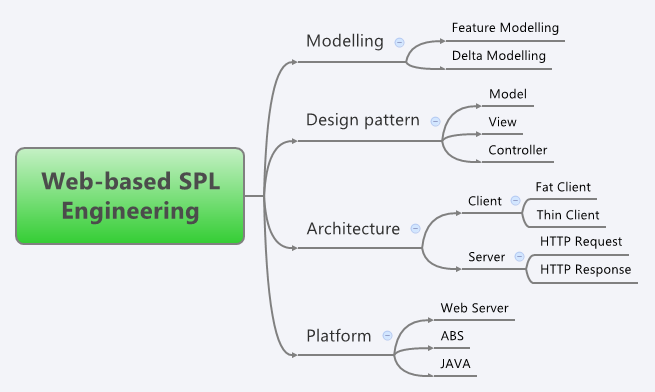
\includegraphics[width=0.8\textwidth]
        {img/kerangka-berpikir.png}
    \caption{Kerangka berpikir}
\end{figure}

\noindent
Setelah penulis mengetahui solusi apa yang harus digunakan agar ABS dapat berjalan di \textit{Application Server}, selanjutnya penulis akan merancang bagaimana pengorganisasian kode yang baik untuk ABS agar sesuai dengan kaidah MVC. Hal ini perlu dilakukan karena nantinya penelitian ini akan menghasilkan sebuah \textit{framework} MVC yang akan digunakan dalam pengembangan SPL berbasis web dengan menggunakan ABS. Dalam hal ini, penulis harus mengkaji terkait peran-peran setiap komponen pada MVC dan kemudian mengimplementasikannya ke ABS. \\

\noindent
Rangkaian proses diatas diharapkan nantinya menghasilkan sebuah framwork MVC yang utuh untuk kemudian diintegrasikan dengan konsep \textit{feature modelling} dan \textit{delta modelling} yang ada di ABS. Hal ini dilakukan agar dapat dihasilkan sebuah framework MVC ABS yang dapat digunakan untuk keperluan pengembangan SPL berbasis web.

%---------------------------------------------------------
\section{Sistematika Penulisan}
%---------------------------------------------------------
berikut adalah sistematika penulisan dari proposal ini:
\begin{itemize}
    \item Bab 1 Pendahuluan \\
    Bab ini berisi tentang latar belakang penelitian, manfaat penelitian, kerangka berpikir, dan sistematika penulisan.
    \item Bab 2 Studi Literatur \\
    Bab ini berisi tentang hasil studi literatur yang dilakukan oleh penulis baik terkait teori-teori dasar yang mendukung penelitian ini ataupun peneletian lain yang masih berkaitan dengan penelitian yang akan dilakukan.
    \item Bab 3 Rumusan Masalah \\
    Bab ini berisi tentang rumusan masalah dari penelitian yang akan dilakukan, ruang lingkup penelitian, serta batasan penelitian.
    \item Bab 4 Rancangan Penelitian \\
    Bab ini berisi tentang rancangan penelitian yang akan dilakukan oleh penulis dan penjelasan dari setiap tahapan-tahapan yang akan dilakukan.
\end{itemize}
\include{RumusanMasalah}
\chapter{Hasil Studi Literatur}

%---------------------------------------------------------
\section{Model View Controller}
%---------------------------------------------------------
\noindent
\textit{Model-View-Controller} (MVC) atau yang biasa juga dikenal dengan sebutan \textit{Presentation-Abstraction-Control} (PAC) merupakan salah satu pendekatan dalam proses pengembangan perangkat lunak yang ditujukan untuk melakukan pemisahan antara logika aplikasi, data, dan presentasi. Konsep ini dibangun atas kesadaran bahwa sebuah model domain aplikasi yang sama dapat disajikan dan diperlakukan secara berbeda tergantung dari kebutuhan si pengguna aplikasi. Dengan menggunakan pendekatan ini, seorang pengembang perangkat lunak dapat berfokus pada satu bagian saja tanpa harus mengkhawatirkan akan terkena dampak perubahan ataupun memberikan perubahan ke bagian aplikasi lainnya.

\subsection{Sejarah Singkat MVC}
\noindent
Konsep MVC diterapkan pertama kalinya oleh Alan Kay, Dan Ingalls, dan Adele Goldberg pada tahun 1980 ketika mereka merancang bahasa pemrograman smalltalk-80 di Xerox PARC Learning Research Group (LRG) \citep{krasner1988desc}. bahasa pemrograman ini didesain dan dikembangkan dengan menggunakan strategi yang merepresentasikan informasi, tampilan, dan kontrol pada lingkungan pemrogramannya. Strategi ini digunakan dengan tujuan (1) untuk membuat kumpulan komponen sistem spesial yang dibutuhkan dalam mendukung proses pengembangan perangkat lunak yang interaktif serta (2) menyediakan kumpulan komponen sistem umum yang dapat membantu pengembang dalam menciptakan aplikasi grafis yang interaktif dengan mudah \citep{krasner1988desc}. Strategi dan tujuan tersebut dibuat dalam rangka menjawab isu utama dalam pengembangan perangkat lunak yaitu terkait pemanfaatan kembali komponen yang telah dibuat (\textit{reusability}) dan kemudahan dalam menggabungkan setiap komponen aplikasi (\textit{plugability}). \\

\noindent
Belajar dari pengalamannya dalam mengembangkan smalltalk-76, para pengembang smalltalk-80 menemukan bahwa untuk mencapai sebuah modularitas yang tinggi diperlukan adanya tiga buah pemisahan fokus dalam pengembangan aplikasi. Tiga buah pemisahan fokus tersebut antara lain adalah (1) memisahkan setiap komponen yang merepresentasikan model domain aplikasi dengan (2) cara yang digunakan untuk merepresentasikan model tersebut ke pengguna aplikasi dan (3) cara yang digunakan oleh pengguna dalam berinteraksi dengan model tersebut. Tiga buah pemisahan tersebut dapat terangkum dalam sebuah konsep yang disebut dengan \textit{Model-View-Controller} (MVC).

\subsection{Penerapan MVC dalam Pengembangan Aplikasi Web}
Aplikasi web merupakan aplikasi yang tergolong interaktif karena aplikasi jenis ini banyak memiliki elemen-elemen yang dapat digunakan untuk berinteraksi dengan penggunannya. Sebagai contoh, dalam sebuah halaman situs web tentunya kita akan menemukan banyak tombol, gambar, tautan, dan kotak isian yang dapat kita gunakan untuk berinteraksi dengan situs web tersebut. Untuk sebuah aplikasi yang tergolong interaktif, adanya pemisahan antara logika aplikasi, data, dan presentasi tentunya akan dapat meningkatkan fleksibilitas aplikasi tersebut dari segi pengembangan. \\

\noindent
Pada dasarnya, arsitektur apliksi berbasis web terbagi menjadi dua bagian yaitu \textit{client} dan \textit{server}. Dengan arsitektur yang seperti ini, para pengembang aplikasi tidak dapat menentukan dengan jelas bagaimana bentuk partisi yang harus dibuat untuk aplikasi tersebut. Sebagai contoh, dengan adanya pembagian antara \textit{client} dan \textit{server}, para pengembang aplikasi harus menentukan dimanakah komponen \textit{view} akan dibentuk? Apakah komponen ini akan dibentuk di tingkat \textit{client} ataukah di tingkat \textit{server}. Begitupun dengan komponen \textit{Model} dan \textit{Controller
}-nya. Apakah komponen-komponen tersebut akan akan dibuat di tingkat \textit{client}, \textit{server}, atau keduanya? Pada akhirnya, keputusan dalam menentukan skema partisi yang dipakai akan sangat bergantung pada teknologi yang digunakan \citep{leff2001web}. \\

\noindent
Permasalahan terkait pemisahan antara \textit{client} dan \textit{server} pada aplikasi berbasis web menjadikan penerapan MVC lebih sulit. Proses penerapan MVC akan dapat berhasil apabila (1) para pengembang aplikasi sudah mengetahui bagaimana skema partisi yang akan diterapkan serta (2) teknologi dan infrastruktur yang ada \textit{compatible} dengan skema partisi yang diterapkan. Oleh karena itu, perlu adanya sebuah pendekatan yang dapat digunakan oleh para pengembang untuk memastikan dua hal tersebut.

%---------------------------------------------------------
\section{Software Product Line Engineering (SPLE)}
%---------------------------------------------------------
\noindent
\textit{Software Product Line Engineering} (SPLE) merupakan sebuah paradigma yang digunakan dalam proses pengembangan perangkat lunak dengan menggunakan prinsip \textit{platform} dan \textit{mass customisation} \citep[p.~14]{pohl2005software}. Dalam industri perangkat lunak, istilah \textit{platform} atau \textit{software platform} biasa diartikan sebagai sebuah sistem komputer (misal: prosesor atau kombinasi antara perangkat keras dengan sistem operasi) yang menyebabkan dapat berjalannya sebuah program komputer. Sedangkan dalam konteks SPLE, yang dimaksud dengan \textit{platform} adalah sebuah subsistem dan \textit{interface} yang membentuk sebuah struktur umum dimana nantinya sebuah produk turunan dapat dikembangkan dan diproduksi secara efisien \citep[p.~15]{pohl2005software}. \\

\noindent
Dalam paradigma SPLE, proses pengembangan perangkat lunak dibagi menjadi dua bagian yaitu \textit{Domain Engineering} dan \textit{Application Engineering} \citep[p.~21]{pohl2005software}. \textit{Domain Engineering} adalah sebuah proses dalam SPLE dimana pada tahap ini seluruh \textit{commonality} dan \textit{variability} dari SPL didefinisikan dan direalisikan. Sedangkan tahap \textit{Application Engineering} adalah sebuah proses dimana aplikasi dari SPL dibuat dengan cara memanfaatkan \textit{domain artifact} yang telah dibuat pada tahap sebelumnya dan mengeksploitasi \textit{variability} yang ada di dalam SPL tersebut. Tahapan-tahapan proses dalam SPLE ini biasa disebut dengan istilah \textit{SPLE Framework}. \\

\begin{figure}
    \centering
    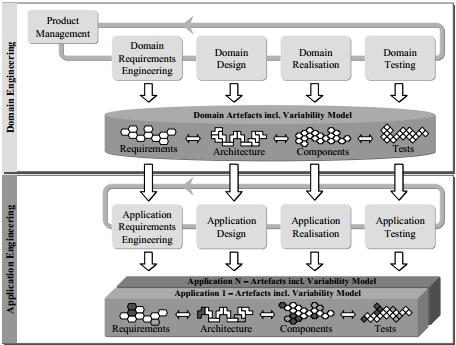
\includegraphics[width=0.8\textwidth]
        {img/sple-process.png}
    \caption{SPLE Framework}
\end{figure}
\vspace{-0.8cm}
\begin{center}
{\small Sumber gambar: \citep{pohl2005software}}
\end{center}

%---------------------------------------------------------
\section{Abstract Behavioural Spesification (ABS)}
%---------------------------------------------------------
\noindent
Abstract Behavioural Specification Language (ABS) merupakan sebuah bahasa pemodelan yang dibuat oleh konsorsium uni eropa di bawah proyek bernama \textit{Highly Adaptable and Trustworthy Software using Formal Method} (HATS). Tujuan dari proyek HATS dalam menciptakan ABS adalah untuk menciptakan sebuah pendekatan yang \textit{model-centric} dalam melakukan proses perancangan, implementasi dan verifikasi dari sebuah sistem yang \textit{highly-configurable} \citep{clarke2012variability}. Pada dasarnya ABS dibagi kedalam beberapa layer (lihat gambar 2.x) yang diantaranya adalah \textit{functional abstraction}, \textit{OO-Imperative layer}, \textit{Concurency Model} dan \textit{ABS Core}. \\

\begin{figure}
    \centering
    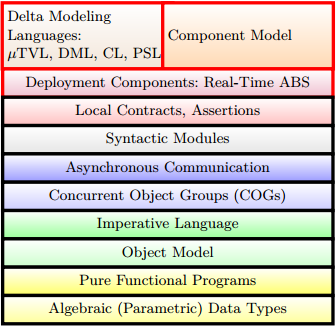
\includegraphics[width=0.6\textwidth]
        {img/abs-layers.png}
    \caption{ABS Layer}
\end{figure}
\vspace{-0.8cm}
\begin{center}
{\small Sumber gambar: \citep{hahnle2013hats}}
\end{center}

\noindent
Sebagai sebuah bahasa pemrograman \textit{imperative} yang menganut konsep \textit{Object Oriented}, secara umum ABS memiliki sintaks yang sama dengan bahasa pemrograman JAVA (walaupun lebih sederhana). Salah satu perbedaan yang paling mendasar antara ABS dengan JAVA adalah pada konsep \textit{code reuse}-nya. Pada bahasa pemrograman JAVA, konsep \textit{code reuse} diimplementasikan dengan cara membuat \textit{code inheritance} sedangkan pada ABS konsep tersebut diimplementasikan dalam betuk \textit{code deltas} \citep{hahnle2013hats}. \textit{code deltas} pada ABS merupakan sebuah kumpulan kode yang mendeskripsikan perubahan-perubahan kode pada kelas yang dituju. Dengan adanya konsep ini, ABS dapat melakukan manipulasi kelas seperti menambah atau menghilangkan \textit{variable} dan \textit{method}. \\

\noindent
Seperti yang sudah disebutkan sebelumnya bahwa di dalam ABS konsep \textit{code reuse} diimplementasikan dalam bentuk \textit{code deltas}. \textit{Code deltas} tersebut nantinya akan digunakan untuk memodelkan \textit{variability} yang terjadi di tingkat \textit{source code}. pemodelan \textit{variability} ini merupakan sebuah pendekatan yang dilakukan oleh ABS dalam membangun sebuah SPL. Proses pemodelan \textit{variability} ini biasa disebut juga sebagai proses \textit{Delta Modelling}. \\

\noindent
\textit{Delta Modelling} merupakan sebuah pendekatan yang fleksible dan modular dalam mewujudkan berbagai macam variasi produk dengan menggunakan kembali artifak-artifak yang ada \citep{hahnle2013hats}. Dalam proses \textit{Delta Modelling}, realisasi dari SPL dibentuk dari dua bagian yaitu \textit{core module} dan \textit{delta module}. \textit{Delta module} berisi fungsi-fungsi yang berlaku umum terhadap semua varian produk yang akan dibuat sedangkan \textit{delta modul} merupakan enkapsulasi dari perubahan-perubahan yang akan terjadi pada \textit{core product} untuk kemudian menghasilkan varian produk yang lain. \\

\begin{figure}
    \centering
    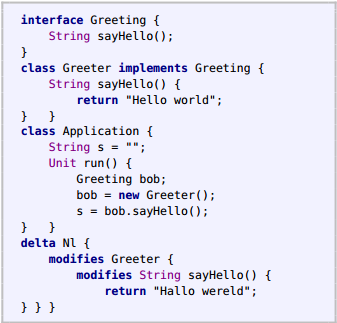
\includegraphics[width=0.6\textwidth]
        {img/delta-modelling-1.png}
\end{figure}

\begin{figure}
    \centering
    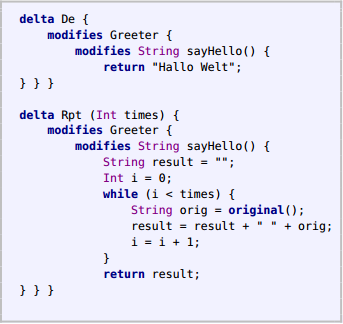
\includegraphics[width=0.6\textwidth]
        {img/delta-modelling-2.png}
    \caption{Delta Modelling pada ABS}
\end{figure}\vspace{-0.8cm}
\begin{center}
{\small Sumber gambar: \citep{clarke2012variability}}
\end{center}
\chapter{Metodologi Penelitian}

Berdasarkan rumusan masalah, ruang lingkup penelitian, serta batasan penelitian yang sudah dibahas pada bab sebelumnya, berikut ini adalah metodologi penelitian yang penulis gunakan:

\begin{figure}
    \centering
    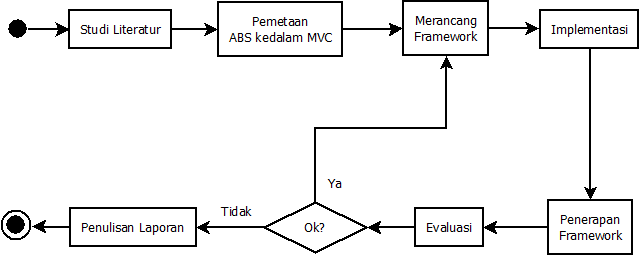
\includegraphics[width=0.8\textwidth]
        {img/metodologi-penelitian.png}
    \caption{Rencana Penelitian}
    \label{fig:metodologiPenelitian}
\end{figure}

Seperti yang terlihat pada Gambar \ref{fig:metodologiPenelitian} diatas, pada awal penelitian penulis melakukan studi literatur untuk mendapatkan pengetahuan terkait teori-teori pendukung yang penulis gunakan dalam melakukan penelitian. Setelah selesai melakukan studi literatur, berikutnya penulis melakukan proses analisa dan pemetaan terhadap bahasa pemodelan ABS untuk kemudian dilakukan pemetaan kedalam komponen-komponen MVC. Seteah proses pemetaan selesai, penulis membuat rancangan ABS MVC Framework sesuai dengan hasil analisa dan pemetaan yang telah dilakukan dan setelah itu penulis melakukan proses implementasi untuk merealisasikan desain yang telah dibuat. Langkah berikutnya adalah melakukan proses penerapan ABS MVC Framework untuk melihat apakah \textit{framework} yang dibuat dapat digunakan untuk membuat sebuah aplikasi berbasis web dan melakukan evaluasi terhadap \textit{framework} tersebut untuk menentukan apakah harus dilakukan perombakan atau sudah layak sebagai sebuah MVC Framework. Berikut ini adalah detail dari setiap tahapan penelitian yang penulis lakukan:

\section{Studi Literatur}

Pada tahap ini penulis melakukan studi literatur dari berbagai sumber seperti buku, artikel ilmian dan web untuk mendapatkan informasi dan pengetahuan terkait teori pendukung yang penulis butuhkan dalam melakukan penelitian ini. Adapun pengetahuan-pengetahuan pendukung yang penulis butuhkan antara lain adalah pengetahuan tentang Hypertext Transfer Protocol (HTTP), pola Model-View-Controller (MVC) dalam pengembangan perangkat lunak, pengetahuan tentang bahasa pemodelan ABS dan pengetahuan tentang \textit{Software Product Line Engineering} (SPLE).

\section{Pemetaan ABS kedalam MVC}

Pada tahap ini penulis melakukan analisa terhadap bahasa pemodelan ABS sesuai dengan pengetahuan yang penulis dapatkan dalam proses studi literatur yang sudah penulis lakukan sebelumnya. Tujuan dari proses analisa yang penulis lakukan ini adalah untuk memetakan bahasa pemodelan ABS kedalam komponen-komponen ABS.

\section{Merancang ABS MVC Framework}

Pada tahap ini penulis membuat rancangan ABS MVC Framework berdasarkan hasil analisa dan pemetaan ABS yang dibuat sebelumnya. Adapun rancangan yang dibuat adalah mengenai bagaimana penyusunan direktori dari \textit{framework} tersebut, bagaiamana karakteristik dari setiap komponen MVC yang dibuat dengan menggunakan ABS serta bagaimana caranya agar komponen MVC yang dibuat dapat menghasilkan sebuah halaman web.

\section{Implementasi}

Pada tahap ini penulis merealisasikan rancangan ABS MVC Framework yang telah penulis buat sebelumnya. Adapun poin-poin implementasi yang dilakukan antara lain adalah mengintegrasikan \textit{framework} ABS yang dibuat dengan JAVA dan \textit{web server} agar \textit{framework} tersebut dapat menghasilkan sebuah halaman web yang utuh.

\section{Penerapan ABS MVC Framework}

Pada tahap ini penulis membuat sebuah aplikasi web dengan menggunakan ABS MVC Framework yang dibuat sekaligus mencoba untuk menerapkan \textit{delta modeling} dan SPLE terhadap \textit{framework} tersebut.

\section{Evaluasi}

Pada tahap ini penulis mengevaluasi hasil penerapan yang dilakukan untuk melihat apakah pelu adanya revisi dan perancangan ulang atau \textit{framework} tersebut sudah sesuai dengan tujuan dari penelitian ini. Apabila hasil evaluasi dari \textit{framework} yang dibuat belum memuaskan, makan akan dilakukan proses revisi rancangan untuk lebih menyempurnakan lagi \textit{framework} yang dibuat. Namun, apabila hasil evaluasi sudah memuaskan maka langkah selanjutnya adalah mendokumentasikan hasil penelitian yang diperoleh kadalam laporan penelitian. Adapun syarat-syarat kelayakan yang penulis tetapkan sebagai parameter keberhasilan dalam proses evaluasi ini antara lain adalah:

\begin{enumerate}
    \item Apakah \textit{framework} yang dihasilkan sudah sesuai dengan kaidah MVC yang berlaku? (sesuai dengan yang ada pada studi literatur)
    \item Apakah \textit{framework} yan dihasilkan dapat diintegrasikan dengan \textit{feature modeling} dan \textit{delta modeling} pada ABS?
    \item Apakah \textit{framework} yang dihasilkan sudah dapat mengasilkan sebuah \textit{complete product} SPL berbasis web? (dapat dijalankan)
\end{enumerate}

\section{Penulisan Laporan}

Pada tahap ini penulis akan menuliskan laporan penelitian dan menarik kesimpulan yang diambil dari penelitian yang sudah dilakukan serta memaparkan temuan-temuan yang diperoleh selama melakukan penelitian.
\chapter{Implementasi}
Bab ini memaparkan secara kronologis tentang proses eksperimen yang telah dilakukan oleh penulis.

\section{Mengintegrasikan ABS dengan JAVA}
Berdasarkan hasil studi literatur yang telah dilakukan, penulis mengetahui bahwa salah satu fitur yang dimiliki oleh ABS adalah kemampuannya untuk dapat di\textit{compile} kedalam bahasa JAVA sehingga nantinya kode ABS tersebut dapat dijalankan di dalam JAVA Runtime Environment (JRE). Berdasarkan informasi tersebut, penulis menarik kesimpulan bahwa jika penulis membuat sebuah JAVA class yang dibuat secara \textit{native}, maka JAVA Class tersebut akan dapat memanggil class ABS yang sudah di\textit{compile} menjadi JAVA Class juga.\\

Sebelum penulis mencoba untuk mengintegrasikan secara langsung ABS dengan JAVA, penulis mencoba untuk mengetahui hasil kompilasi kode ABS yang diubah kedalam JAVA. berikut adalah kode ABS sederhana yang penulis buat beserta hasil kompilasinya ke dalam kode JAVA.

\begin{lstlisting}[
caption=Kode ABS beserta Main Blocknya,
label={lst:absSederhana},
escapeinside={@}{@}
]
module UserModule;

interface User
{
	String getUsername();
}

class UserImpl implements User
{
	String getUsername() @\label{lst:absString}@
	{
		return "salman"; @\label{lst:absString2}@
	}
}

//ABS Main block
{
	User myUser = new local UserImpl(); @\label{lst:absCreateObject}@
	String username = myUser.getUsername();
}
\end{lstlisting}

\begin{lstlisting}[ 
firstnumber=64,
caption=Hasil kompilasi ABS ke JAVA untuk method getUsername(),
label={lst:absjavaGetUsername},
escapeinside={@}{@},
]
// User.abs:10:2: 
public final abs.backend.java.lib.types.ABSString getUsername() {
    ...
    return abs.backend.java.lib.types.ABSString.fromString("salman"); @\label{lst:absjavaString}@
}
\end{lstlisting}

\begin{lstlisting}[
caption=Hasil kompilasi ABS ke JAVA untuk Main Block,
label={lst:absjavaMainBlock},
escapeinside={@}{@}
]
package UserModule;
public class Main extends abs.backend.java.lib.runtime.ABSObject {
    public static void main(java.lang.String[] args) throws Exception {
        abs.backend.java.lib.runtime.StartUp.startup(args,Main.class);
    }
    public java.lang.String getClassName() { return "Main"; }
    public java.util.List<java.lang.String> getFieldNames() { return java.util.Collections.EMPTY_LIST; }
    public Main(abs.backend.java.lib.runtime.COG cog) { super(cog); }
    public abs.backend.java.lib.types.ABSUnit run() {
         {
            ...
            UserModule.User_i myUser = UserModule.UserImpl_c.__ABS_createNewObject(this); @\label{lst:absjavaCreateObject}@
            
            ...
            abs.backend.java.lib.types.ABSString username = abs.backend.java.lib.runtime.ABSRuntime.checkForNull(myUser).getUsername();
            if (__ABS_getRuntime().debuggingEnabled()) __ABS_getRuntime().getCurrentTask().setLocalVariable("username",username);
        }
        
        return abs.backend.java.lib.types.ABSUnit.UNIT;
    }
}
\end{lstlisting}

Seperti yang terlihat pada kode \ref{lst:absjavaMainBlock} baris \ref{lst:absjavaCreateObject}, terdapat perbedaan pada kode JAVA hasil kompilasi dari ABS dalam membuat \textit{instance} dari sebuah objek. Dalam bahasa JAVA yang standar, untuk dapat membuat \textit{instance} dari sebuah class adalah dengan menggunakan kata kunci \texttt{new} seperti misalnya \texttt{new UserImpl()}. Sedangkan pada kode JAVA hasil kompilasi ABS menggunakan kata kunci \texttt{\_\_ABS\_createNewObject(this)} yang diakses secara \textit{static}.\\

Berdasarkan hasil percobaan tersebut penulis mengetahui bahwa sintaks ABS yang terdapat pada kode \ref{lst:absSederhana} baris \ref{lst:absCreateObject} adalah \textit{equivalent} dengan sintaks JAVA yang terdapat pada kode \ref{lst:absjavaMainBlock} baris \ref{lst:absjavaCreateObject}. Dengan demikian, penulis dapat menyimpulkan bahwa ketika penulis ingin mencoba untuk memanggil class JAVA hasil kompilasi ABS dari class JAVA yang \textit{native} maka penulis harus melakukan pemanggilan fungsi seperti yang terlihat pada kode kode \ref{lst:absjavaMainBlock} baris \ref{lst:absjavaCreateObject} tersebut.\\

Selain terdapat perbedaan dalam cara membuat \textit{instance} dari sebuah class, terdapat pula perbedaan pada tipe data yang digunakan oleh JAVA hasil kompilasi dari ABS dengan JAVA yang \textit{native}. Jika kita melihat kode \ref{lst:absSederhana} baris \ref{lst:absString} dan \ref{lst:absString2} penulis menggunakan sebuah tipe data \texttt{String} seperti layaknya tipe data \texttt{String} pada JAVA. Akan tetapi ketika kode ABS tersebut di\textit{compile} kedalam bahasa JAVA, ternyata tipe data \texttt{String} tersebut diubah menjadi \texttt{ABSString} seperti yang terlihat pada kode \ref{lst:absjavaGetUsername} baris \ref{lst:absjavaString}. Berdasarkan hasil percobaan tersebut penulis berkesimpulan bahwa ketika penulis ingin mengintegrasikan ABS dengan JAVA, penulis perlu melakukan konversi tipe data dari tipe data milik JAVA ABS menjadi tipe data standar JAVA.\\

Kesimpulan yang penulis dapatkan setelah melakukan percobaan ini adalah: (1) bahwa untuk dapat membuat sebuah \textit{instance} dari class JAVA hasil kompilasi ABS tidak dapat dilakukan dengan menggunakan kata kunci \texttt{new} seperti pada JAVA yang \textit{native} dan (2) terdapat perbedaan tipe data antara \textit{native} JAVA dengan JAVA hasil kompilasi ABS sehingga perlu adanya penyesuaian lebih lanjut agar penulis dapat mengintegrasikan ABS dengan \textit{native} JAVA.

\section{Membuat halaman web sederhana menggunakan ABS}
Setelah penulis melakukan percobaan sederhana untuk mengetahui cara mengintegrasikan ABS dengan JAVA, selanjutnya penulis melakukan percobaan untuk dapat membuat halaman web sederhana dengan menggunakan ABS. Seperti yang telah kita ketahui bersama, untuk dapat menampilkan sebuah halaman web pada web browser, dibutuhkan adanya sebuah web server yang nantinya akan dapat melayani permintaan dari web browser. Dalam percobaan ini penulis membuat sebuah web server sederhana dengan menggunakan \texttt{ServerSocket} pada JAVA untuk membuka \textit{port} dan menerima \textit{request} dari \textit{web browser} yang nantinya akan memanggil class JAVA hasil kompilasi ABS untuk mendapatkan halaman web yang diinginkan (lihat gambar \ref{fig:howAbsGenerateHTML}).

\begin{figure}
    \centering
    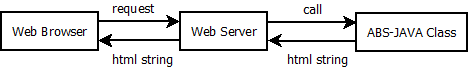
\includegraphics[
        width=0.8\textwidth
    ]{img/request-webserver-abs.png}
    \caption{Bagaimana web server menghasilkan sebuah halaman web}
    \label{fig:howAbsGenerateHTML}
\end{figure}

Untuk dapat mensimulasikan proses seperti yang telah digambarkan pada gambar \ref{fig:howAbsGenerateHTML} di atas, pertama-tama penulis membuat sebuah ABS Module yang fungsinya adalah untuk dapat menghasilkan sebuah halaman sederhana dan memberikannya kepada \textit{web server}. berikut adalah kode ABS yang penulis buat untuk menghasilkan sebuah halaman web:

\begin{lstlisting}[
caption=Kode ABS untuk menghasilkan halaman HTML,
label={lst:absWelcomeView},
]
module ABS.MVC.View.WelcomeView;

interface WelcomeView
{
	String generateView();
}

class WelcomeViewImpl implements WelcomeView
{
	
	String generateView() {		
		String html = "<!DOCTYPE HTML>";
		html = html + "<html>";
		html = html + "<body>";
		html = html + "<h1>Welcome!!</h1>";
		html = html + "Please login <a href='/login.abs'>here</a>";
		html = html + "<br />";
		html = html + "<p>This page was generated from ABS Class</p>";
		html = html + "</body>";
		html = html + "</html>";
		
		return html;
	}
}
\end{lstlisting}

Seperti yang terlihat pada kode \ref{lst:absWelcomeView} di atas, penulis menggunakan \texttt{String} berisikan kode HTML yang disambung-sambung (\textit{concatted String}) untuk menghasilkan sebuah halaman web. Rencananya adalah string yang sudah dihasilkan oleh halaman ABS Module ini nantinya akan diberikan ke \textit{web server} untuk kemudian diberikan ke \textit{web browser} dan ditampilkan ke \textit{user}. Sebagai awalan, penulis membuat sebuah class JAVA yang ditujukan untuk memanggil class JAVA hasil kompilasi ABS tersbut untuk kemudian ditampilkan di \textit{console} dengan menggunakan \texttt{System.out.println()}. Berikut adalah kode JAVA yang dibuat oleh penulis beserta hasil pemanggilan class ABS-nya.

\begin{lstlisting}[
caption=Kode JAVA untuk memanggil ABS,
label={lst:javaCallABS},
escapeinside={@}{@}
]
package com.fmse.absserver;

public class ABSMain extends ABSObject 
{
    ...
       
    public ABSUnit run() {
        System.out.println("ABSMain running..");
        WelcomeView_i view = WelcomeViewImpl_c.__ABS_createNewObject(this); @\label{lst:javaCreateABSObject}@
        ABSString html = ABSRuntime.checkForNull(view).generateView(); @\label{lst:javaCallABSMethod}@
        System.out.println(html.getString());
        return ABSUnit.UNIT; 
    }
    
    public static void main(String[] args) throws Exception {
        StartUp.startup(new String[0], ABSMain.class);
    }
}
\end{lstlisting}

\begin{figure}
    \centering
    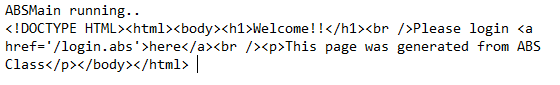
\includegraphics[
        width=0.8\textwidth
    ]{img/java-call-abs-result.png}
    \caption{Hasil dari pemanggilan ABS yang berisikan HTML String}
    \label{fig:javaABSCallResult}
\end{figure}

Terlihat pada kode \ref{lst:javaCallABS} baris \ref{lst:javaCreateABSObject} dan \ref{lst:javaCallABSMethod} di atas, penulis membuat sebuah \textit{instance} dari class \texttt{WelcomView} serta melakukan pemanggilan fungsi \texttt{generateView()} untuk mendapatkan \texttt{String} HTML yang telah dibuat. Hasil dari pemanggilan fungsi \texttt{generateView()} pada class \texttt{WelcomeView} tersebut adalah sebuah \texttt{String} panjang berisikan kode HTML seperti yang terlihat pada gambar \ref{fig:javaABSCallResult}.\\

Setelah penulis berhasil memanggil class JAVA hasil kompilasi ABS untuk mendapatkan HTML String, langkah selanjutnya adalah memberikan HTML String tersebut kepada web browser. Untuk dapat melakukan hal tersebut, penulis akan membuat sebuah web server sederhana dengan menggunakan class \texttt{ServerSocket} pada JAVA. Berikut adalah kode JAVA yang penulis buat untuk dapat menerima request dari \textit{web browser} dan memberikan halaman web yang diinginkan kepada \textit{web browser}.

\begin{lstlisting}[
caption=Potongan kode web server yang memanggil class ABS,
label={lst:javaSimpleWebServer},
escapeinside={@}{@}
]
public class ABSHttpServer extends ABSObject {

    ...
    
    public ABSUnit run() {
        try {
            ServerSocket serverSocket = new ServerSocket(8080); @\label{lst:javaCreateSocket}@
            while(true) {
                Socket remote = serverSocket.accept(); @\label{lst:javaCreateSocket2}@
                BufferedReader in = new BufferedReader(
                        new InputStreamReader(remote.getInputStream()));
                String request = in.readLine();
                String[] protocols = request.split(" ");
                
                ...
                
                if(protocols[1].equals("/")) { @\label{lst:serverStartCallABS}@
                	WelcomeView_i view = WelcomeViewImpl_c.__ABS_createNewObject(this); 
                    html = ABSRuntime.checkForNull(view).generateView().getString();
                    out.println(html);
                } @\label{lst:serverEndCallABS}@
                
                out.flush();
                remote.close();
            }
        }
        catch(Exception e) {
            e.printStackTrace();
        }
        
        return ABSUnit.UNIT;
    }
    
    ...
}
\end{lstlisting}

Pada kode \ref{lst:javaSimpleWebServer} baris \ref{lst:javaCreateSocket} dan \ref{lst:javaCreateSocket2} di atas, terlihat bahwa penulis melakukan pembuatan \texttt{ServerSocket} dan membuka \textit{port} 8080 untuk menerima \textit{request} dari \textit{web browser}. Setelah \textit{web server} menerima \textit{request} dari \textit{web browser}, berikutnya \textit{web server} akan mencocokan URL yang diberikan oleh \textit{web browser} seperti yang terlihat pada gambar \ref{fig:webBrowserRequest}. Apabila URL yang diminta cocok dengan salah satu kondisi yang ada di \textit{web server}, berikutnya \textit{web server} akan melakukan pemanggilan class ABS seperti yang terlihat pada kode \ref{lst:javaSimpleWebServer} baris \ref{lst:serverStartCallABS} - \ref{lst:serverEndCallABS}. Setelah HTML String berhasil diterima oleh \textit{web server} berikutnya akan diberikan ke \textit{web browser} melalui \texttt{OutputStream} pada \texttt{ServerSocket} untuk kemudian ditampilkan di \textit{web browser} seperti yang terlihat pada gambar di bawah ini.

\begin{figure}
    \centering
    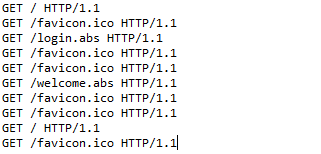
\includegraphics[
        width=0.6\textwidth
    ]{img/web-browser-request.png}
    \caption{Contoh \textit{request} dari \textit{web browser}}
    \label{fig:webBrowserRequest}
\end{figure}

\begin{figure}
    \centering
    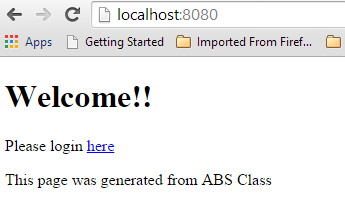
\includegraphics[
        width=0.6\textwidth
    ]{img/abs-welcome-view.png}
    \caption{Halaman web yang dibuat menggunakan ABS}
    \label{fig:javaABSCallResult}
\end{figure}

Sampai pada tahap ini penulis telah berhasil membuat sebuah halaman web sederhana dengan menggunakan ABS. Langkah berikutnya yang penulis lakukan adalah mencoba untuk memetakan ABS kedalam komponen-komponen MVC untuk membuat sebuah MVC Framework.

\section{Memetakan ABS kedalam komponen MVC}
Salah satu tujuan dibentuknya framework MVC untuk ABS adalah agar para pengembang perangkat lunak dapat dengan mudah memisahkan kode program yang mengandung logika bisnis, data dan presentasi dari sebuah aplikasi. Oleh karena itu, sebelum membentuk sebuah framework MVC secara utuh, penulis perlu melakukan pemetaan terhadap kode ABS kedalam setiap komponen Model, View dan Controller (MVC). Tujuan dari dilakukannya proses pemetaan ini adalah agar penulis mendapatkan gambaran bagaimana seharusnya komponen Model, View dan Controller tersebut dibuat dengan menggunakan ABS.\\

Secara umum ABS memiliki sintaks yang tidak jauh berbeda dengan JAVA. Selain itu ABS juga sudah mendukung model pemrograman Object-Oriented Programming (OOP). Oleh karenanya penulis dapat menggunakan pengalaman penulis dalam menggunakan framework MVC untuk JAVA dan PHP (karena keduanya memiliki konsep OOP) beserta hasil studi literatur yang sudah penulis lakukan dalam melakukan proses pemetaan ini. Jika kita merujuk pada publikasi yang dibuat oleh \cite{krasner1988desc} dan \cite{leff2001web} tentang MVC, berikut adalah karakteristik dari masing-masing komponen MVC:

\begin{itemize}
    \item Model: merupakan bagian dari aplikasi yang merepresentasikan data pada aplikasi dan memiliki fungsi yang dapat digunakan untuk memanipulasi data sesuai dengan input yang diberikan.
    \item View: merupakan bagian dari aplikasi yang berfungsi untuk menampilkan informasi kepada user baik dalam bentuk teks ataupun grafis.
    \item Controller: merupakan bagian dari aplikasi yang berfungsi untuk menerima, mengintepretasikan dan memproses setiap \textit{input} yang diberikan oleh \textit{user}.
\end{itemize}

Berdasarkan karakteristik di atas apabila penulis ingin membuat sebuah halaman web yang menampilkan sebuah daftar data mahasiswa (berisikan nomor mahasiswa, nama dan alamat) dalam bentuk tabel, maka komponen-komponen aplikasi yang harus penulis buat antara lain adalah (1) sebuah ABS module yang dapat merepresentasikan data mahasiswa (Model), (2) sebuah ABS module yang dapat menampilkan data mahasiswa dalam bentuk tabel (View) dam (3) sebuah ABS module yang berfungsi untuk mengintegrasikan kedua module tersebut (Controller). Berikut ini adalah module-module ABS yang penulis buat berdasarkan rincian tersebut:

\begin{lstlisting}[
caption=Module ABS untuk merepresentasikan data mahasiswa,
label={lst:absModuleMahasiswa}
]
module MMahasiswa;
export Mahasiswa, MahasiswaImpl;

interface Mahasiswa
{
	String getNpm();
	String getNama();
	String getAlamat();
}

class MahasiswaImpl(
	String npm, String nama, String alamat) implements Mahasiswa
{
	String getNpm() { return this.npm; }
	String getNama() { return this.nama; }
	String getAlamat() { return this.alamat; }
}
\end{lstlisting}

Seperti yang terlihat pada kode \ref{lst:absModuleMahasiswa} di atas, penulis membuat sebuah module ABS yang hanya berisikan atribut npm, nama dan alamat beserta method accessor-nya (\texttt{getNpm()}, \texttt{getNama()} dan \texttt{getAlamat()}). Module ini dibuat hanya mengandung atribut dan \textit{accessor} adalah karena untuk dapat merepresentasikan data Mahasiswa, module ini harus menyimpan atribut-atribut yang berhubungan dengan Mahasiswa beserta dengan \textit{method} pembantu untuk melakukan manipulasi data sesuai dengan input yang diberikan \textit{user}.\\

Setelah berhasil membuat komponen Model \texttt{Mahasiswa}, berikutnya adalah membuat komponen View yang akan menampilkan data mahasiswa dalam bentuk tabel. Berikut adalah kode ABS yang dibuat oleh penulis dalam membuat komponen View tersebut:

\begin{lstlisting}[
caption=Module ABS untuk menampilkan data Mahasiswa dalam bentuk tabel,
label={lst:absModuleMhsView}
]
module MMahasiswaListView;
export MahasiswaListView, MahasiswaListViewImpl;
import Mahasiswa, MahasiswaImpl from MMahasiswa;

interface MahasiswaListView
{
	String generateView();
}

class MahasiswaListViewImpl
	(List<Mahasiswa> listMhs) implements MahasiswaListView
{
	String generateView()
	{
		String html = "<!DOCTYPE HTML>";
		html = html + "<html>";
		html = html + "<body>";
		html = html + "<h1>Daftar Mahasiswa</h1>";
		html = html + "<table>";
		html = html + "<thead>";
		html = html + "<tr>";
		html = html + "<td>No.</td>";
		html = html + "<td>NPM</td>";
		html = html + "<td>Nama</td>";
		html = html + "<td>Alamat</td>";
		html = html + "</tr>";
		html = html + "<tbody>";
		
		Int listLength = length(listMhs);
		Int index = 0;
		while(index < listLength)
		{
			Mahasiswa mhs = nth(listMhs, index);
			String npm = mhs.getNpm();
			String nama = mhs.getNama();
			String alamat = mhs.getAlamat();
			Int nomor = index + 1;
			
			html = html + "<tr>";
			html = html + "<td>" + toString(nomor) + "</td>";
			html = html + "<td>" + npm + "</td>";
			html = html + "<td>" + nama + "</td>";
			html = html + "<td>" + alamat + "</td>";
			html = html + "</tr>";
			index = index + 1;
		}
		
		html = html + "</tbody>";
		html = html + "</table>";
		
		return html;
	}
}
\end{lstlisting}

Kode \ref{lst:absModuleMhsView} di atas merupakan module ABS yang dibuat berdasarkan kriteria komponen View pada MVC yang sudah penulis bahas sebelumnya. Dikarenakan komponen View hanya berfungsi untuk menampilkan data yang diberikan, maka module ABS ini hanya berisi sebuah \textit{method} untuk menghasilkan sebuah halaman HTML yang akan menampilkan daftar mahasiswa.\\

Sampai tahap ini penulis sudah membuat module ABS yang merepresentasikan data Mahasiswa (kode \ref{lst:absModuleMahasiswa}), selain itu penulis juga sudah membuat sebuah module ABS yang dapat menghasilkan sebuah halaman HTML untuk menampilkan data-data mahasiswa dalam bentuk tabel (kode \ref{lst:absModuleMhsView}). Selanjutnya, penulis akan membuat satu buah module lagi yang tersisa yaitu module ABS yang bertugas untuk mengintegrasikan kedua buah module yang sudah dibuat sebelumnya. Berikut adalah kode ABS yang penulis buat untuk merealisasikan hal tersebut:

\begin{lstlisting}[
caption=Module ABS untuk mengintegrasikan antara data dan presentasi,
label={lst:absModuleMhsController},
escapeinside={@}{@}
]
module MMahasiswaController;
import MahasiswaListView, MahasiswaListViewImpl from MMahasiswaListView;
import Mahasiswa, MahasiswaImpl from MMahasiswa;

interface MahasiswaController
{
	String showMahasiswaList();
}

class MahasiswaControllerImpl 
	implements MahasiswaController
{
	String showMahasiswaList()
	{
		List<Mahasiswa> listMhs = Nil; @\label{lst:absStartCreateMhsList}@
		Mahasiswa andi = new local MahasiswaImpl(
		"1306001", "Andi", "Jl. Depok Baru");
		
		Mahasiswa budi = new local MahasiswaImpl(
		"1306002", "Budi", "Jl. Mampang Raya");
		
		Mahasiswa cita = new local MahasiswaImpl(
		"1306003", "Cita", "Jl. Irian Jaya");
		
		listMhs = appendright(listMhs, andi);
		listMhs = appendright(listMhs, budi);
		listMhs = appendright(listMhs, cita); @\label{lst:absEndCreateMhsList}@
		
		MahasiswaListView view = 
			new local MahasiswaListViewImpl(listMhs); @\label{lst:absGenerateMhsView}@
		
		String html = view.generateView(); @\label{lst:absGenerateMhsView2}@
		
		return html;
	}
}
\end{lstlisting}

Seperti yang terlihat pada kode \ref{lst:absModuleMhsController} di atas, module tersebut berperan dalam mengintegrasikan modul \texttt{Mahasiswa} dengan modul \texttt{MahasiswaListView} untuk menghasilkan sebuah halaman web yang berisi daftar mahasiswa dalam bentuk tabel. Pada kode \ref{lst:absModuleMhsController} baris \ref{lst:absStartCreateMhsList} - \ref{lst:absEndCreateMhsList} penulis membuat tiga buah objek \texttt{Mahasiswa} yang kemudian penulis masukan kedalam sebuah \texttt{List} yang merupakan representasi dari data-data Mahasiswa. Selanjutnya penulis memberikan data tersebut ke dalam objek \texttt{MahasiswaListView} untuk kemudian ditampilkan dalam bentuk HTML seperti yang tertera pada kode \ref{lst:absModuleMhsController} baris \ref{lst:absGenerateMhsView} dan \ref{lst:absGenerateMhsView2}.\\

Setelah berhasil membuat tiga buah modul yang dibutuhkan, berikutnya penulis akan memanggil modul \texttt{MahasiswaController} untuk melihat hasil dari halaman web yang dibuat. Oleh karena itu penulis menambahkan sedikit kode pada web server yang penulis buat (lihat kode \ref{lst:javaSimpleWebServer}) untuk memanggil module \texttt{MahasiswaController} tersebut. berikut adalah tambahan kode yang telah penulis buat beserta halaman web yang telah berhasil dibuat dengan menggunakan ABS.

\begin{lstlisting}[
caption=Tambahan kode pada web server untuk memanggil modul \texttt{MahasiswaController},
label={lst:javaCallMahasiswaController}
]
else if(protocols[1].equals("/listMahasiswa"))
{
    MahasiswaController_i controller = MahasiswaControllerImpl_c.__ABS_createNewObject(this);
    html = ABSRuntime.checkForNull(controller).showMahasiswaList().getString();
    out.println(html);
}
\end{lstlisting}

\begin{figure}
    \centering
    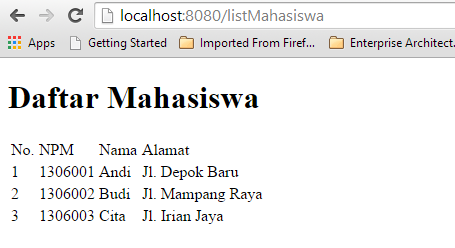
\includegraphics[
        width=0.6\textwidth
    ]{img/hasil-list-mhs.png}
    \caption{Halaman daftar mahasiswa yang dibuat menggunakan ABS}
    \label{fig:htmlDaftarMhs}
\end{figure}

Sampai pada tahap ini, penulis telah berhasil memetakan modul-modul ABS yang dibuat kedalam komponen MVC untuk menghasilkan sebuah halaman web. Namun penulis masih menemukan banyak kekurangan dalam pembuatan komponen MVC ini yang salah satu diantaranya adalah ketika kita membuat komponen view (modul \texttt{MahasiswaListView}). Jika melihat kode \ref{lst:absModuleMhsView} di atas, kode HTML yang dibuat oleh penulis masih berupa \texttt{String} yang disambung-sambung. Hal ini tentunya sangat tidak efektif terlebih lagi jika penulis ingin membuat sebuah halaman web yang lebih kompleks. Oleh karena itu, dibutuhkan adanya solusi lain untuk dapat membuat komponen view ini menjadi lebih mudah dibuat dan dikelola.

\section{Memperbaiki komponen view menggunakan HTML Template Engine}

Berdasarkan hasil evaluasi pada percobaan sebelumnya, penulis merasa perlu untuk mengganti metode yang penulis lakukan dalam membuat komponen view dengan menggunakan ABS. Setelah dikaji lebih jauh lagi, penulis menyadari bahwa standar yang berlaku dalam membuat sebuah halaman web adalah dengan menggunakan HTML. Pada saat penulis membuat komponen view dengan menggunakan ABS untuk menghasilkan HTML, proses pembuatan komponen view menjadi lebih rumit dan kurang fleksibel. Oleh karena itu, penulis membuat keputusan untuk meninggalkan ABS dan beralih ke kode HTML murni ketika membuat komponen view aplikasi.\\

Salah satu pendekatan yang dapat dilakukan utuk mengintegrasikan ABS dengan HTML adalah dengan menggunakan HTML \textit{template engine}. Secara singkat HTML \textit{template engine} adalah sebuah perangkat lunak yang dapat digunakan para pengembang perangkat lunak untuk dapat menyematkan objek ke dalam sebuah HTML dengan menggunakan sintaks tambahan. Dengan menggunakan perangkat lunak ini, penulis dapat langsung menyematkan modul \texttt{Mahasiswa} yang telah penulis buat kedalam sebuah halaman HTML. Dalam penelitian ini, penulis menggunakan HTML \textit{template engine} berbasis JAVA yaitu Thymeleaf (http://thymeleaf.org).

\begin{figure}
    \centering
    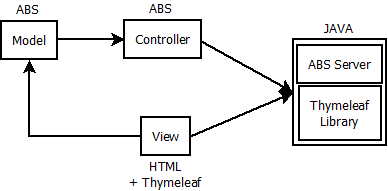
\includegraphics[
        width=0.8\textwidth]{img/alur-thymeleaf.png}
    \caption{Integrasi ABS, JAVA dan Thymeleaf}
    \label{fig:integrasiThymeleaf}
\end{figure}

Seperti yang terlihat pada gambar \ref{fig:integrasiThymeleaf}, dalam kasus ini penulis tidak langsung memanggil komponen View melalui Controller seperti yang penulis lakukan pada kode \ref{lst:absModuleMhsController}. Hal ini dilakukan karena komponen View yang dibuat dengan menggunakan thymeleaf murni menggunakan sintaks HTML sehingga tidak dapat dibuat objeknya. Penggunaan HTML dalam membuat komponen View tentunya akan mempermudah para pengembang perangkat lunak dalam membuat komponen View serta memubuat komponen view menjadi lebih rapih dan mudah dibaca. berikut perubahan pada komponen view yang penulis buat dengan menggunakan thymeleaf:

\begin{lstlisting}[
caption=Komponen View menggunakan HTML dan Thymeleaf,
label={lst:viewMhsListHTML},
escapeinside={@}{@}
]
<!DOCTYPE html>
<html>
<body>
	<h1>Daftar Mahasiswa</h1>
	<table>
		<thead>
			<tr>
				<td>No.</td>
				<td>NPM</td>
				<td>Nama</td>
				<td>Alamat</td>
			</tr>
		</thead>
		<tbody>
			<tr th:each="mahasiswa: ${mahasiswaList}">
				<td><p th:text="${#ids.seq('')}"></p></td>
				<td><p th:text="${mahasiswa.npm}"></p></td>
				<td><p th:text="${mahasiswa.nama}"></p></td>
				<td><p th:text="${mahasiswa.alamat}"></p></td>
			</tr>
		</tbody>
	</table>
</body>
</html>
\end{lstlisting}

Seperti yang terlihat pada kode \ref{lst:viewMhsListHTML} di atas, penulis membuat sebuah halaman web yang equivalent dengan kode \ref{lst:absModuleMhsView} hanya saja kode ini dibuat dengan menggunakan sintaks HTML dan thymeleaf. Jika kita lihat kode \ref{lst:viewMhsListHTML} baris \ref{lst:thymeStartLoop} - \ref{lst:thymeEndLoop} terdapat sebuah sintaks yang bukan standar HTML, sintaks tersebut merupakan sintaks dari thymeleaf (bisanya dintadi dengan \texttt{th:}). Tujuan dari penggunaan sintaks tersebut adalah untuk melakukan iterasi pada sebuah \texttt{List} untuk kemudian menampilkan seluruh atribut dari objek yang berada di dalam \texttt{List} tersebut.\\

Sampai pada tahap ini penulis telah berhasil memperbaiki komponen view dari yang sebelumnya menggunakan ABS menjadi HTML dan thymeleaf sehingga membuat komponen ini menjadi lebih mudah untuk didefinisikan dan lebih sesuai dengan kebiasaan para pengembang. Akan tetapi perubahan ini belum dapat diintegrasikan secara langsung dengan komponen-komponen lainnya karena masih banyak penyesuaian yang harus dilakukan baik di tingkat \textit{web server} maupun di komponen MVC lainnya. Oleh karena itu, langkah selanjutnya yang dilakukan oleh penulis adalah mengubah \textit{web server} dan komponen MVC lainnya agar sesuai dengan implementasi komponen View yang terbaru.

\section{Mengintegrasikan Thymeleaf dengan Web Server dan ABS}

Walaupum ABS dapat dikompilasi kedalam bentuk JAVA dan Thymeleaf juga merupakan komponen perangkat lunak yang berbasis JAVA, penulis tidak dapat mengintegrasikan dua hal tersebut secara langsung di dalam Class JAVA hasi kompilasi ABS. Hal ini terjadi karena penulis tidak ingin melakukan modifikasi terhadap Class JAVA tersebut dikarenakan Class JAVA ini merupakan \textit{auto generated file} sehingga kodenya akan selalu berubah. Oleh karena itu, penulis memutuskan untuk mengintegrasikan Thymeleaf dengan komponen MVC ABS di tingkat \textit{web server}. berikut adalah langkah-langkah yang penulis ambil dalam proses integrasinya:

\begin{enumerate}
    \item Pada saat \textit{web server} menerima \textit{request} dari \textit{web browser}, \textit{web server} akan memanggil komponen Controller ABS (yang sudah dikompilasi menjadi JAVA) yang diinginkan.
    \item Komponen Controller tersebut nantinya akan memberikan data (komponen Model) dan lokasi berkas HTML yang menjadi komponen View-nya.
    \item Setelah \textit{web server} menerima data dan lokasi berkas HTML dari komponen Controller, selanjutnya \textit{web server} akan mencari berkas HTML tersebut dan membuat sebuah \texttt{Context} untuk kemudian digabungkan dengan data yang diberikan.
    \item Setelah proses penggabungan selesai dan halaman web yang diinginkan sudah terbentuk, selanjutnya \textit{web server} akan memberikan halaman web tersebut kepada web browser.
\end{enumerate}

Berikut adalah modul \texttt{MMahasiswaController} yang sudah diubah sesuai dengan rencana implementasi di atas:

\begin{lstlisting}[
caption=Module \texttt{MMahasiswaController} yang disesuaikan untuk integrasi thymeleaf,
label={lst:absMhsControllerNew},
escapeinside={@}{@}
]
module Controller.MMahasiswaController;
import Mahasiswa, MahasiswaImpl from Model.MMahasiswa;

interface MahasiswaController
{
	Pair<String, List<Mahasiswa>> showMahasiswaList(); @\label{lst:absReturnType}@
}

class MahasiswaControllerImpl implements MahasiswaController
{
	Pair<String, List<Mahasiswa>> showMahasiswaList() @\label{lst:absReturnType2}@
	{
		...
		
		return Pair("list_mahasiswa", listMhs); @\label{lst:absReturnViewAndModel}@
	}
}
\end{lstlisting}

Terlihat pada kode \ref{lst:absMhsControllerNew} baris \ref{lst:absReturnViewAndModel}, penulis tidak lagi membuat \textit{instance} dari \texttt{MahasiswaListView} melainkan hanya mengembalikan lokasi berkas HTML yang menjadi komponen View-nya berserta dengan data Mahasiswa yang akan ditampilkan kedalam halaman web. Selain itu, pada bari \ref{lst:absReturnType} dan \ref{lst:absReturnType2} juga terdapat perubahan kode yaitu dari yang sebelumya \textit{method} \texttt{showMahasiswaList} hanya mengembalikan nilai \texttt{String} berubah menjadi \texttt{Pair(String, List<Mahasiswa>)}.

Setelah melakukan perubahan pada komponen Controller, berikutnya adalah melakukan perubahan pada \textit{web server}. Berikut adalah perubahan-perubahan pada web server yang penulis lakukan untuk mengintegrasikan thymeleaf dengan ABS:

\begin{lstlisting}[
caption=Perubahan pada kode \textit{web server},
label={lst:javaNewWebServer}
]
...

else if(protocols[1].equals("/listMahasiswa")) {
   	MahasiswaController_i controller = MahasiswaControllerImpl_c.__ABS_createNewObject(this);
   	Pair<ABSString, ABS.StdLib.List<Mahasiswa_i>> pair = controller.showMahasiswaList();
   	String view = pair.getArg(0).toString().replaceAll("\"", "");
   	
   	ABS.StdLib.List<Mahasiswa_i> absData = (ABS.StdLib.List<Mahasiswa_i>) pair.getArg(1);
   	ArrayList<Object> data = new ArrayList<Object>();
           		
	do
	{
		ABSObject head = (ABSObject) ABS.StdLib.head_f.apply(absData);
		data.add(head);
		
		absData = ABS.StdLib.tail_f.apply(absData);
	}
	while(!(absData instanceof ABS.StdLib.List_Nil));
	
	TemplateResolver templateResolver = new TemplateResolver();
    templateResolver.setTemplateMode("XHTML");
    templateResolver.setSuffix(".html");
    templateResolver.setResourceResolver(new ResourceResolver());
                
    TemplateEngine templateEngine = new TemplateEngine();
    templateEngine.setTemplateResolver(templateResolver);
                
	Context ctx = new Context();
	StringWriter writer = new StringWriter();
	ctx.setVariable("mahasiswaList", data);
	templateEngine.process(view, ctx, writer);
	
	out.println(writer);
}

...
\end{lstlisting}

\begin{lstlisting}[
caption=Class \texttt{ResourceResolver} sebagai tambahan pada \textit{web server},
label={lst:javaResourceResolver}
]
public class ResourceResolver implements IResourceResolver
{
	private static final String NAME = "ABSResourceResolver";
	
	@Override
	public String getName() 
	{
		// TODO Auto-generated method stub
		return NAME;
	}

	@Override
	public InputStream getResourceAsStream(TemplateProcessingParameters templateProcessingParameter,
			String resourceName) 
	{
		
		Validate.notNull(resourceName, "Resource name cannot be null");
		return ResourceResolver.class.getResourceAsStream("/" + resourceName);
	}

}
\end{lstlisting}

\section{Membuat Ant Script untuk mempermudah proses Compile dan Deployment}
Bagian ini menjelaskan tentang proses pembuatan ant script untuk mempermudah proses compile dan deployment dari yang sebelumnya menggunakan menu di eclipse menjadi ke terminal console.

\section{Menerima input POST dan GET dari web browser}
Bagian ini menjelaskan tentang eksperimen yang dilakukan oleh penulis dalam mencari tahu metode seperti apa yang dapat digunakan dalam menerima input HTTP POST dan GET dari web browser.

\section{Membuat Routing configuration}
Bagian ini menjelaskan tentang proses pembuatan routing configuration untuk memetakan setiap url kedalam class controller dan methodnya.
\chapter{Evaluasi dan Analisa ABS MVC Framework}

Bab ini berisi tentang hasil analisis dan evaluasi dari MVC Framework yang telah dibuat. Dalam melakukan proses evaluasi, penulis membandingkan proses yang dilakukan dalam membuat perangkat lunak berbasis web antara menggunakan ABS MVC Framework dengan menggunakan framework lain. Adapun aplikasi web yang digunakan dalam proses evaluasi ini adalah aplikasi web yang telah penulis buat pada bagian penerapan ABS MVC Framwork (aplikasi katalog produk). Framework lain yang penulis gunakan dalam proses evaluasi ini adalah Play Framework (JAVA MVC Framework) versi 2.3 \footnote{https://playframework.com/download}. Berikut ini adalah poin-poin yang akan dievaluasi pada bab ini:

\begin{enumerate}
    \item Evaluasi proses penerapan Model-View-Controller.
    \item Evaluasi proses penanganan perubahan \textit{requirement}.
    \item Evaluasi penerapan SPL dengan menggunakan ABS MVC Framework.
\end{enumerate}

\section{Evaluasi Penerapan Model-View-Controller}

Dalam proses pengembangan apalikasi web dengan menggunakan MVC \textit{framework}, setiap kode yang dibuat akan dikelompokan kedalam komponen Model-View-Controller. Oleh karena itu, untuk mengevalusi framework ABS MVC yang dibuat penulis membandingan proses pembuatan komponen-komponen MVC tersebut antara Play Framework dengan ABS MVC Framework. Berikut adalah hasil evaluasi dan analisa ABS MVC Framework dari poin penerapan MVC-nya.

\subsection{Proses Pembuatan Komponen Model}

Komponen model merupakan komponen yang merepresentasikan entitas data pada aplikasi. Dalam banyak MVC Framework, komponen model dapat diintegrasikan dengan peragkat lunak basis data sehingga setiap komponen model yang dibuat akan merepresentasikan setiap tabel yang ada di dalam basis data. Dalam konteks ABS MVC Framework, proses integrasi komponen model dengan perangkat lunak basis data belum dapat dilakukan seperti yang sudah dibahas pada bagian batasan penelitian. Berikut ini adalah perbandingan antara komponen Model yang dibuat dengan menggunakan ABS MVC Framework dengan Play Framework.

\begin{lstlisting}[
caption=Komponen Model menggunakan ABS,
label={lst:modelUsingABS}
]
interface Product
{
    ...
}

class ProductImpl 
	(String sku, String name, String description, String price) implements Product
{
	String getSku() { return this.sku; }
	String getName() { return this.name; }
	String getDescription() { return this.description; }
	String getPrice() { return this.price; }
	Unit setSku(String sku) { this.sku = sku; }
	Unit setName(String name) { this.name = name; }
	Unit setDescription(String description) { this.description = description; }
	Unit setPrice(String price) { this.price = price; }
}
\end{lstlisting}

\begin{lstlisting}[
caption=Komponen Model menggunakan Play Framework,
label={lst:modelUsingPlay},
escapeinside={!}{!}
]
@Entity !\label{lst:modelAnotasi}!
public class Product extends Model
{
	@Id !\label{lst:modelAnotasi2}!
	public Long id;
	public String sku;
	public String name;
	public String description;
	public Long price;

	public Product(String sku, String name,
		String description, Long price)
	{
		this.sku = sku;
		this.name = name;
		this.description = description;
		this.price = price;
	}

	public static Finder<Long,Product> find = new Finder<Long,Product>( !\label{lst:modelPlayFinder}!
    Long.class, Product.class); 
}
\end{lstlisting}

Seperti yang terlihat pada Kode \ref{lst:modelUsingABS} dan \ref{lst:modelUsingPlay} diatas, kedua buah komponen Model tersebut tidak memiliki perbedaan yang signifikan. keduanya hanya berisikan atribut-atribut yang merepresentasikan data produk pada aplikasi web yang dibuat. Hanya saja, pada komponen model yang dibuat dengan menggunakan Play Framework memiliki tambahan anotasi (bari \ref{lst:modelAnotasi} dan \ref{lst:modelAnotasi2}) serta tambahan \textit{method} (baris \ref{lst:modelPlayFinder}) yang digunakan oleh Play Framework untuk mengintegrasikan komponen tersebut dengan perangkat lunak basis data.\\

Walaupun terdapat beberapa perbedaan antara komponen model yang dibuat dengan ABS Framework dengan Play Framework, akan tetapi kedua komponen tersebut masih memiliki karakteristik yang sama yaitu hanya terdiri dari atribut data dan tidak mengandung proses bisnis aplikasi. Hal ini sejalan dengan definisi komponen Model yang dipaparkan oleh \cite{krasner1988desc} dan \cite{leff2001web} pada publikasi penelitiannya. Dengan demikian, penulis berkesimpulan bahwa metode yang digunakan pada ABS MVC Framework sudah sesuai dengan karakteristik komponen model pada \textit{framework} yang umum digunakan dan juga sudah sesuai dengan landasan teori yang ada.

\subsection{Proses Pembuatan Komponen View}

Dalam banyak \textit{framework} MVC, pembuatan komponen View umumnya menggunakan sintaks HTML dengan tambahan sintaks \textit{template engine} untuk dapat mengintegrasikan antara komponen View tersebut dengan komponen Model yang dibuat. Dalam konteks ABS MVC Framework, komponen View yang dibuat sudah menggunakan sintaks HTML dan \textit{template engine} Thymeleaf sedangkan Play Framewerk juga sudah menggunakan HTML dan \textit{template engine} Twirl. Berikut ini adalah perbandingan komponen View yang dibuat dengan menggunakan ABS MVC Framework dan Play Framework.

\begin{lstlisting}[
caption=Halaman \texttt{list.html} yang dibuat menggunakan Thymeleaf,
label={lst:viewThymeleaf},
escapeinside={!}{!}
]
...
<tbody>
	<tr th:each="product: ${dataList}"> !\label{lst:thymeDataList}!
		<td th:text="${#ids.seq('')}"></td>
		<td th:text="${product.sku}"></td>
		<td th:text="${product.name}"></td>
		<td th:text="${product.price}"></td>
		<td>
			<a th:href="@{http://localhost:8080/product/update.abs(sku=${product.sku})}">update</a>&nbsp;&nbsp;
			<a th:href="@{http://localhost:8080/product/delete.abs(sku=${product.sku})}">delete</a>
		</td>
	</tr>
</tbody>
...
\end{lstlisting}

\begin{lstlisting}[
caption=Halaman \texttt{list.html} yang dibuat menggunakan Twirl,
label={lst:viewTwirl},
escapeinside={!}{!}
]
@(products: List[Product]) !\label{lst:twirlDefineVariable}!
...
<tbody>
	@for((product, index) <- products.zipWithIndex){
		<tr>
			<td>@{index+1}</td>
			<td>@product.sku</td>
			<td>@product.name</td>
			<td>@product.price</td>
			<td>
				<a href="/product/update/@product.sku">update</a>&nbsp;&nbsp;
				<a href="/product/delete/@product.sku">delete</a>
			</td>
		</tr>
	}
</tbody>
...
\end{lstlisting}

Seperti yang terlihat pada Kode \ref{lst:viewThymeleaf} dan \ref{lst:viewTwirl}, kedua komponen View tersebut tidak jauh berbeda dikarenakan keduanya dibuat dengan menggunakan sintaks HTML. Hal yang membedakan dari kedua komponen tersebut terletak pada sintaks \textit{template engine} yang digunakan seperti misalnya pada ABS MVC Framework menggunakan \texttt{\$\{data.sku\}} untuk mendapatkan nomor sku dari objek model yang diberikan, sedangkan Play Framework menggunakan sintaks \texttt{@product.sku}. Perbedaan sintaks ini adalah wajar dikarenakan \textit{template engine} yang digunakan oleh kedua \textit{framework} tersebut adalah berbeda.\\

Walaupun kedua komponen di atas hampir sama, namum komponen View yang dibuat oleh komponen ABS MVC Framework banyak memiliki keterbatasan jika dibandingkan dengan komponen View yang dibuat dengan menggunakan Play Framework. berikut adalah beberapa keterbatasan yang dimiliki oleh ABS MVC Framework:

\begin{itemize}
    \item Memerlukan konvensi khusus untuk dapat memanggil komponen model yang diberikan seperti misalnya penggunaan variable \texttt{dataList} (Kode \ref{lst:viewThymeleaf} barsi \ref{lst:thymeDataList}) untuk objek model berbentuk list dan \texttt{data} (Kode \ref{lst:htmlUpdateProduct}) untuk objek model yang berdiri sendiri. Hal ini berbeda dengan komponen View pada Play Framework yang dapat didefinisikan sendiri oleh pengembang (Kode \ref{lst:viewTwirl} baris \ref{lst:twirlDefineVariable}).
    \item Komponen View pada ABS MVC Framework belum dapat menangani banyak komponen Model yang artinya ketika pengembang membuatuhkan Model Product dan Customer untuk ditampilkan di halaman web,  hal ini belum dapat dilakukan. Berbeda dengan komponen View pada Play Framework yang dapat menerima banyak model dengan menggunakan \texttt{@\(product: Product, customer: Customer\)}.
\end{itemize}

Berdasarkan hasil evaluasi diatas, penulis menyimpulkan bahwa untuk komponen View yang dibuat menggunakan ABS MVC Framework, sudah memiliki karakteristik yang sama dengan komponen yang dibuat menggunakan Play Framework. Akan tetapi, masih terdapat beberapa keterbatasan yang dimiliki sehingga tingkat fleksibilitasnya masih rendah dibandingkan dengan komponen View yang dibuat dengan menggunakan Play Framework.

\subsection{Proses Pembuatan Komponen Controller}

Secara umum fungsi dari komponen Controller adalah mengintegrasikan komponen Model dan View agar dapat dihasilkan sebuah halaman web yang dapat ditampilkan ke pengguna aplikasi. Dalam implementasinya, komponen Controller berisi bisnis proses aplikasi yang didalamnya melakukan pemrosesan \textit{input} yang diberikan oleh pengguna aplikasi. Dalam konteks ABS MVC Framework, kedua hal tersebut sudah dapat dilakukan walaupun dengan mekanisme yang sedikit berbeda dengan komponen Controller yang dibuat dengan menggunakan Play Framework. Berikut ini adalah cuplikan \textit{method} \texttt{saveUpdateProduct} yang ada di dalam Controller ABS MVC Framework dan Play Framework:

\begin{lstlisting}[
caption=Method \texttt{saveUpdateProduct} menggunakan ABS MVC Framework,
label={lst:saveUpdateABS}
]
...
Pair<String, List<Product>> saveUpdateProduct(ABSHttpRequest request)
{
	ProductDB db = new local ProductDBImpl();
	db.init();
	
	String sku = request.getInput("product_sku");
	String name = request.getInput("product_name");
	String description = request.getInput("description");
	String price = request.getInput("price");
	
	Product p = db.findBySku(sku);
	p.setName(name);
	p.setDescription(description);
	p.setPrice(price);
	db.update(p);
	
	List<Product> products = db.findAll();
	return Pair("product/list", products);
}
...
\end{lstlisting}

\begin{lstlisting}[
caption=Method \texttt{saveUpdateProduct} menggunakan Play Framework,
label={lst:saveUpdatePlay}
]
public static Result saveUpdateProduct()
{
    DynamicForm requestData = Form.form().bindFromRequest();
    String sku = requestData.get("product_sku");
    String name = requestData.get("product_name");
    String description = requestData.get("description");
    Long price = Long.parseLong(requestData.get("price"));

    List<Product> products = Product.find.where().eq("sku", sku).findList();
    Product product = products.get(0);
    product.name = name;
    product.description = description;
    product.price = price;
    product.update();

    return ok(list.render(Product.find.all()));
}
\end{lstlisting}

Seperti yang terlihat pada Kode \ref{lst:saveUpdateABS} dan \ref{lst:saveUpdatePlay} diatas, secara umum apa yang dilakukan oleh kedua buah \textit{method} tersebut adalah sama yaitu (1) menerima input dari pengguna aplikasi, (2) melakukan pencarian kedalam basis data untuk mendapatkan produk dengan nomor sku yang sesuai, (3) Mengubah data produk tersebut dengan data yang diberikan oleh pengguna aplikasi dan (4) menampilkan seluruh data produk kedalam halaman \texttt{list.html}. Satu hal yang membedakan kedua komponen Controller diatas adalah pada ABS MVC Framework basis data yang digunakan masih merupakan basis data \textit{dummy} sedangkan pada Play Framework, penulis sudah menggunakan MySQL sebagai basis datanya. Hal ini terjadi karena saat ini, ABS masih belum dapat melakukan akses kedalam basis data sungguhan seperti yang sudah dipaparkan pada bagian batasan penelitian.\\

Selain batasan terkait akses basis data tersebut, terdapat pula keterbatasan lainya yang dimiliki oleh ABS MVC Framework dalam membuat komponen Controller yaitu adalah belum adanya mekanisme yang dapat digunakan oleh ABS MVC Framework untuk memberikan banyak model kedalam komponen View. Hal ini menyebabkan adanya keterbatasan pada komponen View seperti yang dibahas pada bagian evaluasi pembuatan komponen View. Adanya keterbatasan pada komponen Controller dalam memberikan banyak model adalah karena penulis belum menemukan pengganti tipe data \texttt{Generic} yang dimiliki oleh JAVA untuk ABS.\\

Walaupun terdapat beberapa keterbatasan fitur pada komponen Controller ABS MVC Framework, akan tetapi secara karakteristik antara komponen Controller ABS MVC Framework dengan Play Framework tidak jauh berbeda. Sehingga dapat disimpulkan bahwa komponen Controller yang dibentuk dengan menggunakan ABS MVC Framework masih sesuai dengan karakteristik yang dipaparkan oleh \cite{krasner1988desc} dan \cite{leff2001web} serta \textit{framework} MVC lain yang biasa digunakan.

\section{Evaluasi Proses Penanganan Perubahan Requirement}

Perubahan \textit{requirement} terhadap sistem, merupakan satu hal yang tidak dapat dihindari. Dalam konteks ABS MVC Framework, perubahan \textit{requirement} terssebut dapat ditangani dengan membuat kode delta seperti yang penulis bahas pada bab sebelumnya. Dengan menggunakan pendekatan ini, setiap perubahan \textit{requirement} akan tercatat dalam bentuk kode delta yang dibuat sehingga para pengembang memiliki dokumentasi yang jelas terhadap setiap perubahan yang terjadi di dalam sistem. Selain itu, dengan menggunakan pendekatan \textit{delta modelling}, para pengembang aplikasi web dapat dengan leluasa memilih perubahan mana saja yang ingin diimplementasikan tanpa harus kehilangan aplikasi yang aslinya.\\

Lain halnya dengan menggunakan Play Framework, pada saat terjadi perubahan \textit{requirement} pada sistem, mau tidak mau para pengembang aplikasi web tersebut harus melakukan perubahan secara langsung terhadap setiap komponen Model, View dan Controller-nya. Hal ini tentunya akan menyebabkan hilangnya kode aplikasi yang sudah dibuat sebelumnya. Dengan menggunakan pendekatan ini, para pengembang aplikasi web tersebut tidak dapat melacak jejak perubahan yang terjadi pada perangkat lunak yang dibuat dikarenakan setiap perubahan yang terjadi pada sistem langsung berdampak pada kode asli pada sistem tersebut.\\

Berdasarkan pemaparan diatas, dapat diketahui bahwa proses penangan perubahan \textit{requirement} dengan menggunakan pendekatan \textit{delta modelling} memberikan dampak yang lebih baik dibandingkan dengan melakukan perubahan secara langsung terhadap kode aplikasi yang dibuat. Dengan demikian, penulis berpendapat bahwa dalam penangan perubahan \textit{requirement} ini ABS MVC Framework memiliki nilai lebih dibandingkan dengan Play Framework.

\section{Evaluasi penerapan SPL dengan menggunakan ABS MVC Framework}

\textit{Software Product Line Engineering} (SPLE) merupakan sebuah paradigma yang digunakan dalam proses pengembangan perangkat lunak dengan menggunakan prinsip \textit{platform} dan \textit{mass customisation} \citep[p.~14]{pohl2005software}. Dengan menggunakan paradigma ini, para pengembang perangkat lunak dapat menciptakan banyak variasi produk dari produk inti (\textit{core product}) yang dibuat dengan cara melakukan proses perubahan (\textit{customization}) pada produk tersebut. Dalam konteks ABS MVC Framework, proses pembuatan SPLE dapat dilakukan dengan menggunakan pendekatan \textit{delta modelling}. Dengan menggunakan pendekatan ini, para pengembang perangkat lunak dapat menerapkan prinsip \textit{platform} dengan cara membuat \textit{core product} menggunakan kode ABS dan prinsip \textit{mass customization} dengan cara membuat banyak kode delta yang nantinya akan diterapkan di dalam \textit{core product} tersebut untuk dapat menghasilkan banyak variasi produk / \textit{productline}.\\

Sebagai contoh, pada pembahasan sebelumnya penulis telah membuat sebuah perubahan \textit{requirement} pada aplikasi katalog produk yang penulis buat. Perubahan \textit{requirement} tersebut dapat dianggap sebagai sebuah variasi produk dari produk intinya yaitu sebuah aplikasi katalog produk dengan tanpa kategori produk di dalamnya. Dalam kasus ini, penulis memiliki sebuah \textit{productline} yaitu aplikasi web katalog produk yang menyertakan kategori produk di dalamnya. Apabila penulis ingin membuat \textit{productline} yang lain seperti misalnya menambahkan atribut "diskon" pada data produk, penulis cukup membuat kode delta lain dan menambahkannya kedalam konfigurasi produk untuk dapat menghasilkan variasi produk yang baru.\\

Berdasarkan pemaparan tersebut, dapat diketahui bahwa ABS MVC Framework dapat memfasilitasi para pengembang perangkat lunak dalam menghasilkan SPL untuk aplikasi web yang dibuat.


\bibliography{conf/bib}
\bibliographystyle{conf/apalikerd}

\end{document}